\documentclass[10pt]{article} 
\usepackage[margin=2cm]{geometry}
\usepackage{tikz}  

\begin{document}

\title{\textbf{LAB 9 TASK}}

\author{(Ushna Ijaz-2019-CE-39)}
\maketitle

\part*{Pre-Lecture Exercises }

\section*{Question 1}
What algorithmic problem about graphs do we need to solve in order to solve the following
problems? (Note, you do not actually have to solve these problems, just transform them into graph
problems that we might then be able to solve).\\
1. Among actors, a “Bacon number" is the number of degrees of separation from an actor to
Kevin Bacon. For example, Kevin Bacon’s Bacon number is 0. If an actor works in a movie
with Kevin Bacon, the actor’s Bacon number is 1. If an actor A works with an actor B who
worked with Kevin Bacon in a movie, then actor A’s Bacon number is 2, and so forth.\\
(a) What is Samuel L. Jackson’s Bacon number?\\
(b) list all the people with Bacon number equal to 6. 


\section*{Answer}

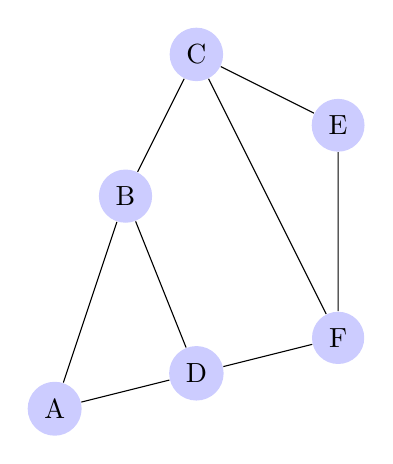
\begin{tikzpicture}  
  [scale=.9,auto=center,every node/.style={circle,fill=blue!20}]  
    
  \node (a1) at (1,2) {A};  
  \node (a2) at (2,5)  {B}; 
  \node (a3) at (3,7)  {C};  
  \node (a4) at (3,2.5) {D};  
  \node (a5) at (5,6)  {E};  
  \node (a6) at (5,3)  {F};  
   
  
  \draw (a1) -- (a2); 
  \draw (a2) -- (a3);  
  \draw (a2) -- (a4);  
  \draw (a4) -- (a6);  
  \draw (a3) -- (a5);  
  \draw (a1)-- (a4);
  \draw (a5) -- (a6);
  \draw (a3) -- (a6);
   
  
\end{tikzpicture}  

\begin{center}
 \begin{tabular}{||c c ||} 
 \hline
 Vertex & Degree  \\ [0.5ex]  
 \hline
 A & 4 \\
 \hline
 B & 3 \\
 \hline
 C & 3  \\
 \hline
 D & 2 \\ 
 \hline
 E & 2 \\
 \hline
 F & 2 \\[1ex] 
 \hline
\end{tabular}
\end{center}



\section*{Question 2}

2. You need to take a bunch of classes at Stanford, and some of them depend on each other.
For example, you must take CS 103 before taking CS 161. Given a set of classes you need
to take, and information about which class is a pre-requisite for which other class, generate
an order in which to take all of the classes. Assume you can only take one class at a time


\section*{Answer}
We will simply use any sorting algorithm to sort it. 
\part*{Homework Questions}

\section*{Question 2}
(a) Run DFS starting at vertex C, breaking any ties by alphabetical order. *\\
a. What do you get when you order the vertices by ascending start time?\\
b. What do you get when you order the vertices by descending finish time?\\
(b) Run DFS starting at vertex C, breaking any ties by reverse alphabetical order.**\\
a. What do you get when you order the vertices by ascending start time?\\
b. What do you get when you order the vertices by descending finish time? 

\section*{Answer }

\subsubsection*{(a)}

a. Ascending starting time: C,D,E,A,B\\
b. Descending finish time: A,B,C,D,E\\
	

\subsubsection*{(b)}
a. Ascending starting time: C,E,D,B,A\\
b. Descending finish time: A,B,C,D,E\\
\end{document} 

 